\section{Results}\label{sec:results}

\begin{table}[t]
\caption{Test results (Llama-3.2-3B, 150 questions). Faults: success under the five answerable
faults (\%). Dmg.: correct clean answers broken (\%). Abst.: abstention when the answer passage is
absent (\%). Tok.: prompt tokens per case.}\label{tab:main}
\small
\begin{tabular}{lrrrr}
\toprule
 & \multicolumn{4}{c}{Llama-3.2-3B} \\
\cmidrule(lr){2-5}
Policy & Faults & Dmg. & Abst. & Tok. \\
\midrule
No repair & 26.8 & 0.0 & 38.7 & 0.7k \\
Retry & 27.6 & 0.0 & 34.0 & 0.9k \\
Self-check (LLM) & 20.7 & 24.3 & 60.7 & 1.5k \\
Self-check (MiniCheck) & 22.4 & 12.1 & 55.3 & 1.0k \\
Repair-all & 46.4 & 15.9 & 20.0 & 2.4k \\
Trace checks only & 55.9 & 1.9 & 38.0 & 1.2k \\
\textbf{Diagnose (text match)} & 56.9 & 4.7 & 28.0 & 1.5k \\
Diagnose (LLM verifier) & 57.2 & 11.2 & 28.0 & 2.3k \\
Diagnose (MiniCheck) & 59.3 & 7.5 & 29.3 & 2.1k \\
\midrule
\quad $-$ re-check & 53.1 & 5.6 & 30.0 & 1.3k \\
\quad $-$ abstention & 59.9 & 1.9 & 23.3 & 1.5k \\
\quad $-$ trace checks & 31.9 & 3.7 & 30.0 & 1.3k \\
\bottomrule
\end{tabular}

\end{table}

\begin{figure*}[t]
\centering
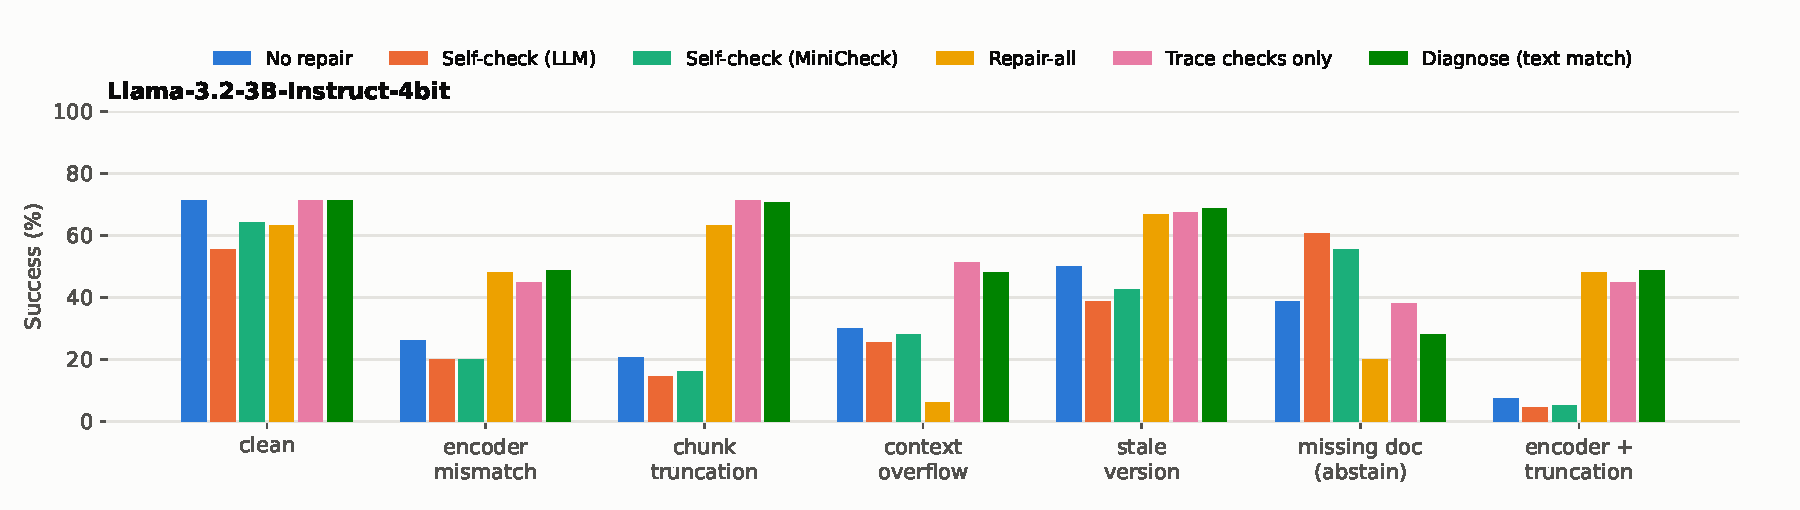
\includegraphics[width=\textwidth]{success_by_condition.pdf}
\caption{Success by condition for six policies (Llama-3.2-3B, 150 test questions). In
\emph{absent}, success means abstaining.}\label{fig:conditions}
\end{figure*}

\subsection{RQ1: Which repairs help?}
Table~\ref{tab:main} and Figure~\ref{fig:conditions} summarize the comparison; all differences
below are paired by question.

\paragraph{Generic repairs do not help.} With no repair the service answers 71.3\% of clean
questions but only 26.8\% [22.7, 31.2] under faults. Retry changes little (27.6\%): it only fires
on \INS{} and resamples the same broken prompt. Self-check is worse than no repair
(20.7\%) and breaks 24.3\% of correct clean answers, almost always by turning them into
\INS{} after its verifier calls them unsupported.

\paragraph{Blanket repair helps but breaks things.} Repair-all (wider dense retrieval plus BM25,
full rendering, newest versions, on every request) reaches 46.4\% under faults. It costs a second
call with 3.6$\times$ the prompt tokens of the deployed pipeline, breaks 15.9\% of correct clean
answers, and lowers abstention on unanswerable questions from 38.7\% to 20.0\%. Under the serving
fault it is far worse than doing nothing (6.0\% vs.\ 30.0\%): its longer prompt loses even more to
the server's silent cut, so the repair amplifies the fault.

\paragraph{Trace checks do most of the work.} The four trace checks with their matching repairs
reach 55.9\% [49.7, 62.0] under faults while breaking 1.9\% of correct clean answers, at 1.72 calls
and 1.2k prompt tokens per case. Diagnose adds a support check, a retrieval ladder and abstention:
56.9\% [50.7, 63.1], +30.1 points over no repair [24.8, 35.7] and +10.5 over Repair-all [6.4, 14.9],
but only +1.1 [$-$2.0, 4.0] over trace checks alone. The ablations explain why. Removing the trace
checks drops success to 31.9\% ($-$25.1 [$-$30.0, $-$20.3]): a support check that sees only the answer
cannot tell a template bug from a retrieval miss, and widening retrieval does not undo truncation or
overflow. Re-checking support after a repair is worth +3.9 points [1.9, 6.0], mostly under the
encoder fault, where the first fallback is often not enough. Abstention costs 2.9 points under
faults [1.1, 5.3] and raises clean damage from 1.9\% to 4.7\%, while recovering only 4.7 points of
appropriate abstention.

\paragraph{The checks are precise.} The truncation and overflow checks fired on every faulty case
and on no clean case; the version check fired on 86\% of stale cases (the outdated copy was in the
prompt in 91\%); the low-retrieval check fired on every encoder-fault case and, by construction of
its threshold, on 4\% of clean cases, where its BM25 fallback did no measurable harm.

\paragraph{Repairs reduce abstention.} When the answer passage is missing, the deployed pipeline
abstains 38.7\% of the time; Diagnose abstains 28.0\% ($p{=}0.004$). The retrieval ladder adds
passages, and the model then finds a plausible but wrong entity to name. Only the self-check
policies abstain more (55--61\%), and they pay for it with clean damage.

\begin{figure}[t]
\centering
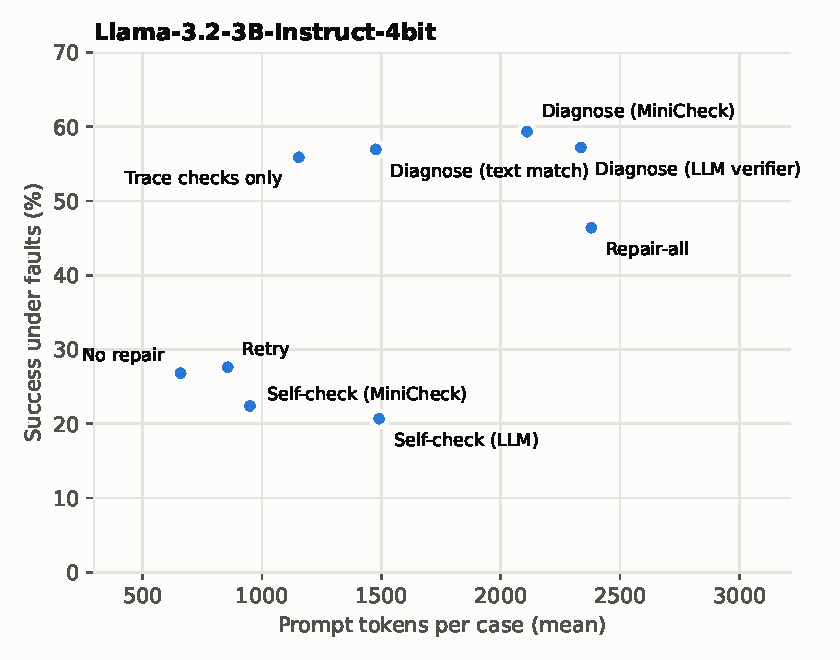
\includegraphics[width=\columnwidth]{cost_vs_success.pdf}
\caption{Success under faults versus prompt tokens per case.}\label{fig:cost}
\end{figure}

\subsection{RQ2: Verifier or repair?}
Table~\ref{tab:factorial} crosses the decision of \emph{whether} an answer is unsupported with
\emph{what happens next}. Regenerating on the same passages fails with either verifier
(20.7\%, 22.4\%); repairing the context succeeds with any of the three (56.9--59.3\%). The repair
action, not the verifier, determines recovery. The verifier mainly determines damage: the LLM
self-verifier breaks the most correct answers in either column.

Table~\ref{tab:support} evaluates the gates directly on 700 non-abstaining initial answers. The LLM
self-verifier keeps only 26.3\% of correct, grounded answers. MiniCheck is better balanced (AUROC
0.67) but still rejects nearly half of the good answers at its default threshold; multi-hop answers
whose support spans two passages are hard for a 355M-parameter grounding classifier.
Is this a small-model artifact? On a stratified sample of 240 of the same answers we asked Claude
Haiku~4.5 the identical verifier question. It keeps 71.7\% of good answers and catches 82.4\% of bad
ones (balanced accuracy 0.77), against 20.7\% and 91.2\% (0.56) for the 3B model's self-verifier and
0.63 for MiniCheck. A stronger verifier would remove most of the false alarms that made self-check
destroy correct answers. It would not make self-check repair anything: under truncation, overflow
or a retrieval fault the evidence is not in the passages, so regenerating on them cannot recover
it, which is what the left column of Table~\ref{tab:factorial} shows for both verifiers. Even the
strong verifier is close to chance on truncated passages (0.53), where the question is whether
missing text would have supported the answer.

\begin{table}[t]
\caption{Verifier $\times$ repair. Cells: success under faults / clean damage (\%).}\label{tab:factorial}
\small
\begin{tabular}{llrr}
\toprule
Model & Verifier & Regenerate & Repair context \\
\midrule
Llama-3.2-3B & LLM self-verifier & 20.7 / 24.3 & 57.2 / 11.2 \\
 & MiniCheck & 22.4 / 12.1 & 59.3 / 7.5 \\
 & Text match & -- & 56.9 / 4.7 \\
\bottomrule
\end{tabular}

\end{table}

\begin{table}[t]
\caption{Support checks as gates on initial answers. Good kept: correct, grounded answers judged
supported. Bad caught: other answers judged unsupported.}\label{tab:support}
\small
\begin{tabular}{lrrr}
\toprule
Check & Good kept & Bad caught & Bal.\ acc. \\
\midrule
\multicolumn{4}{l}{\emph{Llama-3.2-3B: 700 initial answers, 285 correct and grounded}} \\
LLM self-verifier & 26.3 & 86.7 & 0.57 \\
MiniCheck $\geq 0.5$ (AUROC 0.67) & 52.6 & 72.8 & 0.63 \\
\midrule
\multicolumn{4}{l}{\emph{Same 240 answers (40 per condition) for all three}} \\
Llama-3.2-3B self-verifier & 20.7 & 91.2 & 0.56 \\
Claude Haiku 4.5, same prompt & 71.7 & 82.4 & 0.77 \\
MiniCheck $\geq 0.5$ & 45.7 & 81.1 & 0.63 \\
\bottomrule
\end{tabular}

\end{table}

\subsection{RQ3: How fast is a faulty deploy detected?}
We simulate 300 request streams per fault: 400 clean requests, then 200 after a deploy that
introduces the fault (the stale fault affects 20\% of post-deploy requests, the others all of them).
A signal alarms when its rate over the last 50 requests exceeds the clean mean plus three standard
deviations. Table~\ref{tab:monitor} and Figure~\ref{fig:monitor} show that trace checks alarm a
median of 4 requests after each global fault and 24 requests after the partial stale fault, with
0.1\% false alarms. MiniCheck needs 18--35 requests for global faults and rarely detects the stale
one. The LLM verifier flags 75\% of \emph{clean} answers, so its alarm threshold is high; it needs
34--93 requests and misses two thirds of overflow deploys. The model's abstention rate is a
reasonable signal for retrieval and truncation faults (7--10 requests), slow for overflow (56) and
poor for stale documents.

\begin{table}[t]
\caption{Detection delay after a faulty deploy: median requests until the first alarm (share of
300 runs with an alarm). --: detected in fewer than half the runs.}\label{tab:monitor}
\small
\begin{tabular}{lrrrr}
\toprule
Fault & Trace & MiniCheck & LLM ver. & Abstain \\
\midrule
encoder & 4 (100\%) & 23 (100\%) & 63 (67\%) & 10 (100\%) \\
truncation & 4 (100\%) & 19 (100\%) & 39 (92\%) & 10 (100\%) \\
overflow & 4 (100\%) & 35 (100\%) & -- & 56 (89\%) \\
stale & 24 (100\%) & -- & -- & -- \\
enc.+trunc. & 4 (100\%) & 18 (100\%) & 34 (99\%) & 7 (100\%) \\
\bottomrule
\end{tabular}

\end{table}

\begin{figure*}[t]
\centering
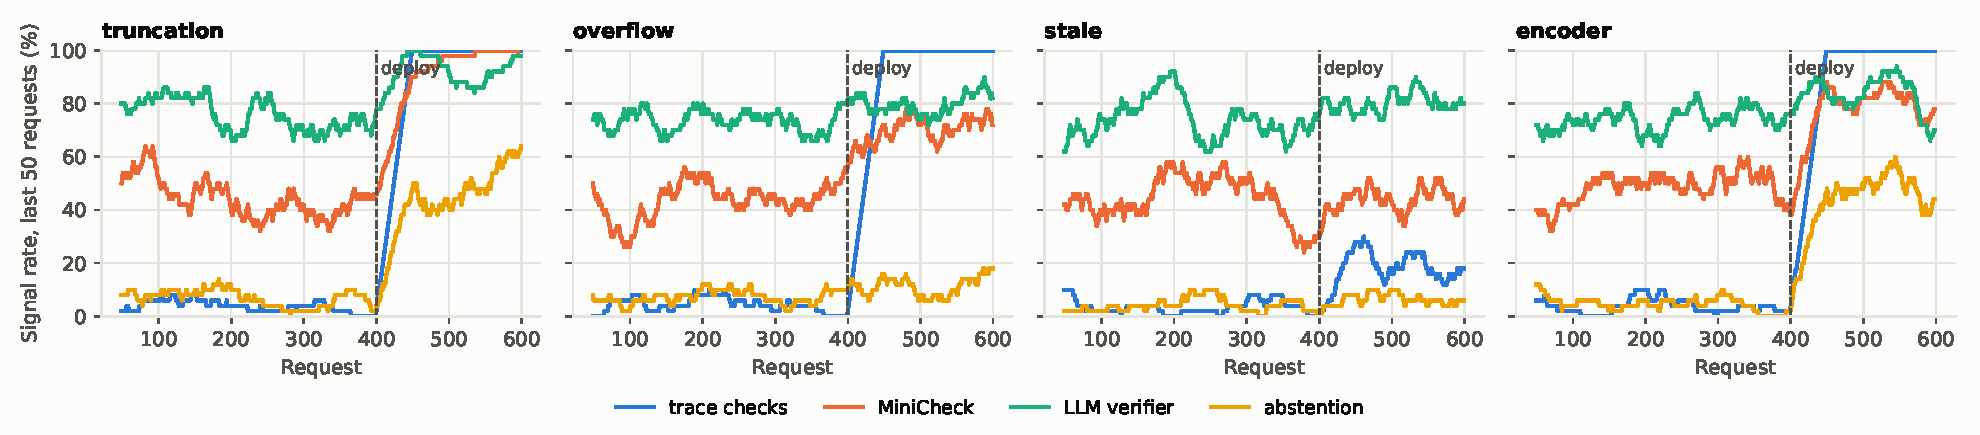
\includegraphics[width=\textwidth]{monitoring_Llama-3.2-3B.pdf}
\caption{Signal rates in one simulated stream per fault; the dashed line marks the deploy.}\label{fig:monitor}
\end{figure*}

\subsection{RQ4: Regression tests from observed failures}
We turned 35 observed cases into a regression suite: five clean questions that must stay correct
and, for each fault, five failures that Diagnose repaired. Because every model response and support
score is cached, the suite replays the full pipeline in about 7 seconds without loading a model;
a code change that alters a prompt or a repair decision misses the cache and fails until it is
re-recorded. To check that the suite has teeth, we disabled one diagnostic at a time and replayed it
on the live model (Table~\ref{tab:mutation}). Every mutation failed exactly the cases of the fault it
covers.

\begin{table}[t]
\caption{Regression suite under mutations of the repair logic (35 cases).}\label{tab:mutation}
\small
\begin{tabular}{lrl}
\toprule
Mutation & Failing & Conditions \\
\midrule
none & 0 & -- \\
no truncation check & 10 & truncation, encoder+truncation \\
no low-retrieval check & 8 & encoder, encoder+truncation \\
no overflow check & 5 & overflow \\
no version check & 4 & stale \\
no re-check after repair & 3 & encoder, encoder+truncation \\
\bottomrule
\end{tabular}
\end{table}

\subsection{Sensitivity to scoring}
The equivalence judge accepted aliases such as ``Bob Iger'' for ``Robert A.\ Iger''. We audited
all 63 of its acceptances on the test set, overturned 13 (it had accepted a related entity, e.g.\
``Greene King'' for ``Bury St Edmunds''), and corrected them; 59 of 60 sampled rejections were
right. With string matching alone, success under faults drops by 8--18 points but every conclusion
holds: Diagnose beats no repair by +24.5 [19.5, 29.9] and Repair-all by +9.9 [5.7, 13.9], trace
checks alone are within +1.3 [$-$0.9, 3.5], and self-check remains the worst policy.
